\documentclass[12pt]{article}
\usepackage[a4paper, total={6in, 8in}]{geometry}
\usepackage{polski}
\usepackage{adjustbox}
\usepackage{pgfplots}
\usepackage{amsmath}
\usepackage{multirow}

\setlength{\parindent}{0pt}
\setlength{\oddsidemargin}{-15pt}
\setlength{\textwidth}{460pt}
\setlength{\textheight}{720pt}

\author{Michał Puchyr, Dawid Chudzicki}
\title{Sprawozdanie z ćw 53 -- PRAWO OHMA DLA PRĄDU PRZEMIENNEGO}

\pgfplotsset{scaled x ticks=false}

\begin{document}
\maketitle

\section{Cel ćwiczenia}
\begin{itemize}
    \item Wyznaczenie wartości indukcyjności cewki i pojemności kondensatora przy zastosowaniu prawa
    Ohma dla prądu przemiennego,
    \item Sprawdzenie prawa Ohma dla prądu przemiennego dla
    szeregowego układu złożonego z opornika, cewki indukcyjnej i kondensatora.
\end{itemize}

\section{Wstęp teoretyczny}

\textbf{Prąd przemienny} (AC) -- charakterystyczny przypadek prądu elektrycznego okresowo zmiennego, 
w którym wartości chwilowe podlegają zmianom w powtarzalny, okresowy sposób, z określoną częstotliwością. 
Wartości chwilowe natężenia prądu przemiennego przyjmują naprzemiennie wartości dodatnie i ujemne. 

Największe znaczenie praktyczne mają prąd i napięcie o przebiegu sinusoidalnym. W żargonie technicznym nazwa prąd przemienny często oznacza po prostu \textbf{prąd sinusoidalny}. \bigskip

\textbf{Kondensator} -- element elektroniczny bierny zbudowany z dwóch przewodników -- inaczej okładek lub elektrod -- 
rozdzielonych dielektrykiem; przechowuje on energię w postaci pola elektrycznego.

Pojemność kondensatora mierzy zdolność kondensatora do magazynowania ładunku elektrycznego.

Jednostką pojemności jest farad (F). 

Kondensatory są wykorzystywane w elektronice do różnych celów, na przykład do filtrowania sygnałów, 
magazynowania energii, stabilizacji napięcia, generowania sygnałów i wielu innych zastosowań. \bigskip

\textbf{Cewka indukcyjna} to element elektryczny składający się z przewijanej spirali z drutu lub taśmy ferromagnetycznej, 
który wykorzystuje zjawisko elektromagnetycznej indukcji do magazynowania energii w postaci pola magnetycznego. 

Indukcyjność jest podstawowym parametrem elektrycznym opisującym cewkę. Jednostką indukcyjności jest henr [H].
Prąd płynący w obwodzie wytwarza skojarzony z nim strumień magnetyczny. 


Indukcyjność definiuje się jako stosunek tego strumienia i prądu, który go wytworzył:

$$ L = k \frac{\Phi}{i} $$
Współczynnik $k$ zależy od geometrii układu, a więc między innymi od kształtu cewki, liczby zwojów, grubości użytego drutu. Indukcyjność cewki zależy również od przenikalności magnetycznej rdzenia.

\bigskip
Wykaz przyrządów :
\begin{itemize}
    \item Generator AG 1022F
    \item Woltomierz napięcia przemiennego
    \item Miliamperomierz prądu przemiennego
    \item Zestaw składający się z oporników, cewek indukcyjnych i kondensatorów
\end{itemize}

Oporność badanego opornika : $ R = (157 \pm 3) \Omega $

Oporność cewki indukcyjnej : $ R_{L2} = (0,60 \pm 0,05) \Omega $

Przedział częstotliwości pomiarowej dla pojemności $C_3$ : od 50 Hz do 200Hz

\section{Przykładowe obliczenia}
\subsection{Niepewności mierników}

Niepewność woltomierza

Dla zakresu:
\begin{itemize}
    \item 4V : $ \pm 0,8 \% \ \textrm{rdg} + 3\textrm{dgt}$ \quad dgt $=1$mV
    \item 40V : $ \pm 2.5 \% \ \textrm{rdg} + 5\textrm{dgt} $ \quad dgt $=10$mV
\end{itemize} \bigskip

Np.
$$ u_b(U) = \frac{0,008 \cdot 1,016 + 3 \cdot 0,001}{\sqrt{3}} = 0,00642 \approx 0,0065[V] $$ \bigskip

Niepewność amperomierza (dla prądu zmiennego)

Dla zakresu:
\begin{itemize}
    \item 40 mA : $ \pm 1.5\% \ \textrm{rdg} + 3\textrm{dgt} $ \quad dgt $=10\mu$A
    \item 400 mA : $ \pm 1.5\% \ \textrm{rdg} + 3\textrm{dgt} $ \quad dgt $=100\mu$A
\end{itemize}

Np. 
$$ u_b(I) = \frac{0,015 \cdot 2,090 + 3 \cdot 0,00001}{\sqrt3} = 0,01811 \approx 0,019[mA]$$\bigskip

Niepewność ustalenia częstotliwości generatora:
\begin{itemize}
    \item $ \pm 1\% \ \textrm{rdg} \pm 1 \textrm{Hz} $
\end{itemize}

Np.
$$ u_b(f) = \frac{0,01 \cdot 125 + 1}{\sqrt{3}} = 1.29903 \approx 1,3[Hz] $$ 

\subsection{Obliczenia prowadzące do wyznaczenia pojemności kondensatora}



\section{Pomiary i opracowanie wyników}

\subsection{Wyznaczanie pojemności kondensatora (RC)}

\begin{center}
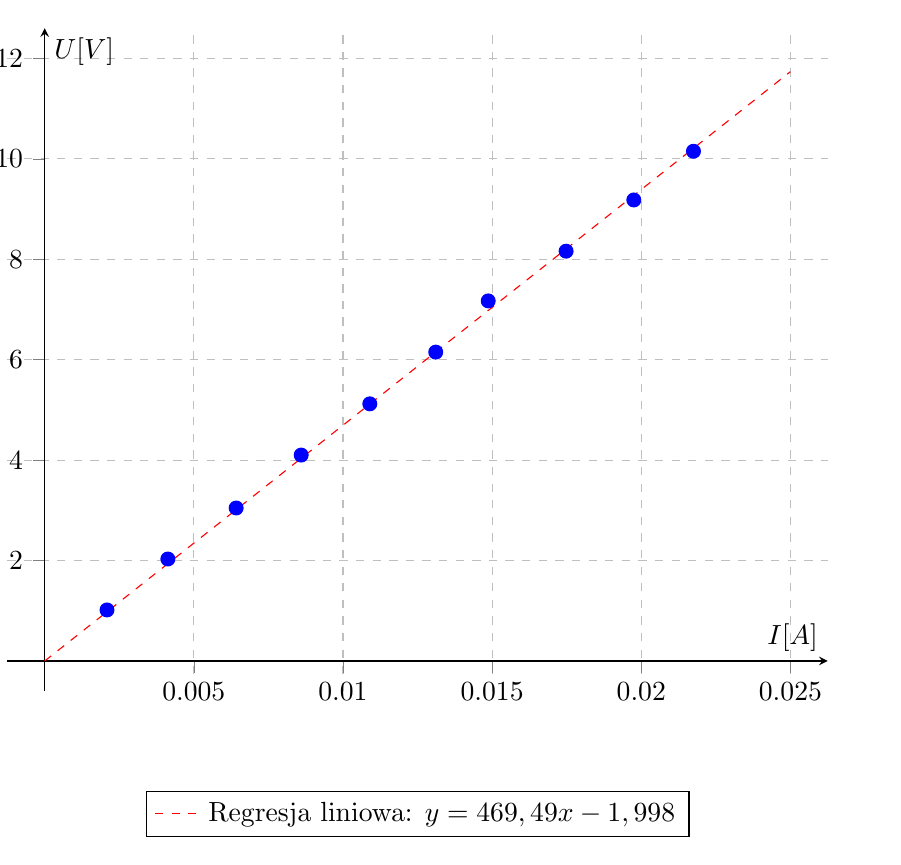
\begin{tikzpicture}
    \begin{axis}[
        xlabel={$I[A]$},
        ylabel={$U[V]$},
        xmin=0,
        xmax=0.025,
        ymin=0,
        ymax=12,
        xtick={0,0.005,0.01,0.015,0.02,0.025},
        ytick={0,2,4,6,8,10,12},
        grid=major,
        grid style={dashed,gray!50},
        width=12cm,
        height=10cm,
        axis lines=middle,
        enlargelimits=0.05,
        tick align=outside,
        legend style={at={(0.5,-0.15)},anchor=north},
        legend cell align=left,
        mark size=2.5pt,
        xticklabel style={
            /pgf/number format/fixed,
            /pgf/number format/precision=5
        },
    ]
    \addplot[red, domain=0:0.025, dashed] {469.49*x-0.001998}; \addlegendentry{Regresja liniowa: $y = 469,49x - 1,998$}
    \addplot[blue, only marks] coordinates {
        (0.00209,1.016)
        (0.00413,2.03)
        (0.00642,3.046)
        (0.0086,4.10)
        (0.0109,5.12)
        (0.01311,6.15)
        (0.01487,7.17)
        (0.01748,8.16)
        (0.01975,9.18)
        (0.02175,10.15)
    };
    \end{axis}
    \end{tikzpicture}

    \textbf{Wykres zależności napięcia od natężenia}
\end{center}

\begin{table}[h]
    \centering
    \caption{Wyniki pomiarów i obliczeń}
    \label{tab:tabela1}
    \begin{tabular}{|c|c|c|c|c|c|c|c|c|c|c|} \hline
    Lp & U[V] & u(U)[V] & I[mA] & u(I)[mA] & Z\textsubscript{c} & u(Z\textsubscript{c}) & $f$[Hz] & u($f$)[Hz] & C & u(C) \\ \hline
    1 & 1,0160 & 0,0065 & 2,090 & 0,019 & \multirow{10}{*}{470} & \multirow{10}{*}{2} & \multirow{10}{*}{125,0} & \multirow{10}{*}{1,3} & \multirow{10}{*}{2,874115$^{-6}$} & \multirow{10}{*}{3,3624$^{-8}$} \\ \cline{1-5}
    2 & 2,034 & 0,012 & 4,130 & 0,036 & & & & & & \\ \cline{1-5}
    3 & 3,046 & 0,016 & 6,420 & 0,056 & & & & & & \\ \cline{1-5}
    4 & 4,100 & 0,089 & 8,600 & 0,075 & & & & & & \\ \cline{1-5}
    5 & 5,12 & 0,11 & 10,900 & 0,095 & & & & & & \\ \cline{1-5}
    6 & 6,15 & 0,12 & 13,11 & 0,12 & & & & & & \\ \cline{1-5}
    7 & 7,17 & 0,14 & 14,87 & 0,13 & & & & & & \\ \cline{1-5}
    8 & 8,16 & 0,15 & 17,48 & 0,16 & & & & & & \\ \cline{1-5}
    9 & 9,18 & 0,17 & 19,75 & 0,18 & & & & & & \\ \cline{1-5}
    10 & 10,15 & 0,18 & 21,75 & 0,19 & & & & & & \\ \hline
    \end{tabular}
\end{table}

\subsection{Wyznaczenie indukcyjności cewki}
    
\end{document}